\begin{figure}[htbp]
    \centering
    \begin{subfigure}{0.24\textwidth}
        \centering
        \includegraphics[width=\linewidth]{data/heat_rotation/0.png}
        \caption{0° Heat=1}
    \end{subfigure}\hfill
    \begin{subfigure}{0.24\textwidth}
        \centering
        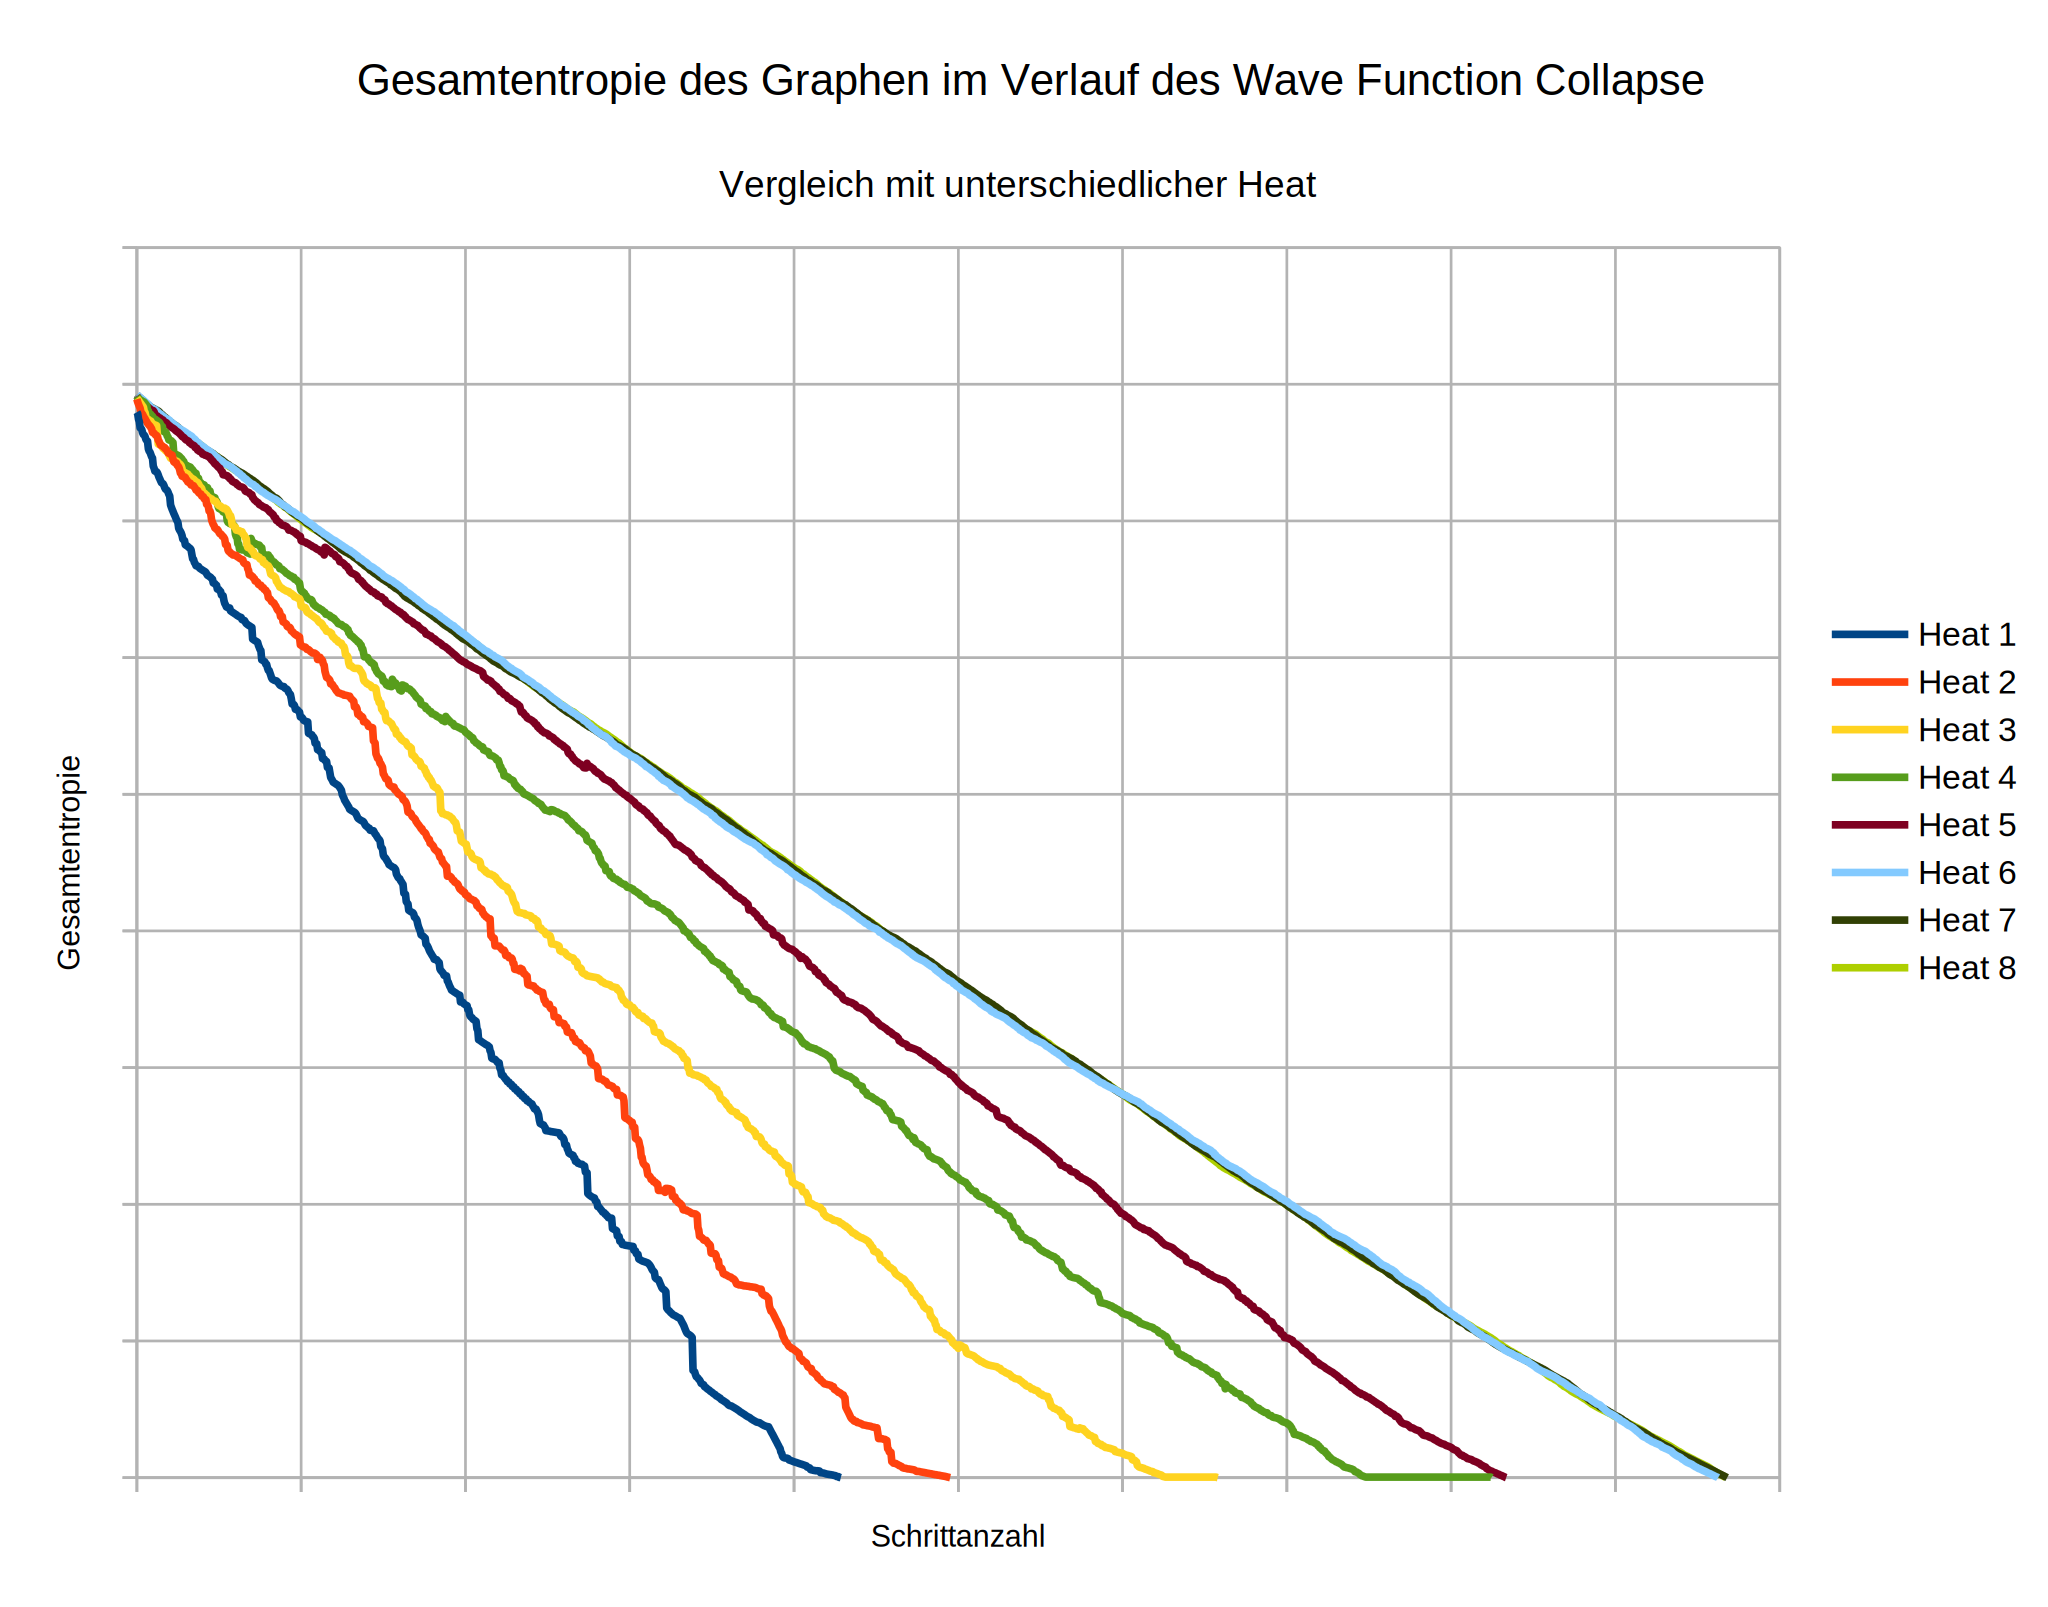
\includegraphics[width=\linewidth]{data/heat_rotation/1.png}
        \caption{22° Heat=1}
    \end{subfigure}\hfill
    \begin{subfigure}{0.24\textwidth}
        \centering
        \includegraphics[width=\linewidth]{data/heat_rotation/2.png}
        \caption{23° Heat=1}
    \end{subfigure}
    \begin{subfigure}{0.24\textwidth}
        \centering
        \includegraphics[width=\linewidth]{data/heat_rotation/3.png}
        \caption{23° Heat=2}
    \end{subfigure}\hfill
    
    \caption{
        Heat als lokale Drehung
    }
    \label{fig:heat_rotation}
\end{figure}